\begin{figure*}
\centering
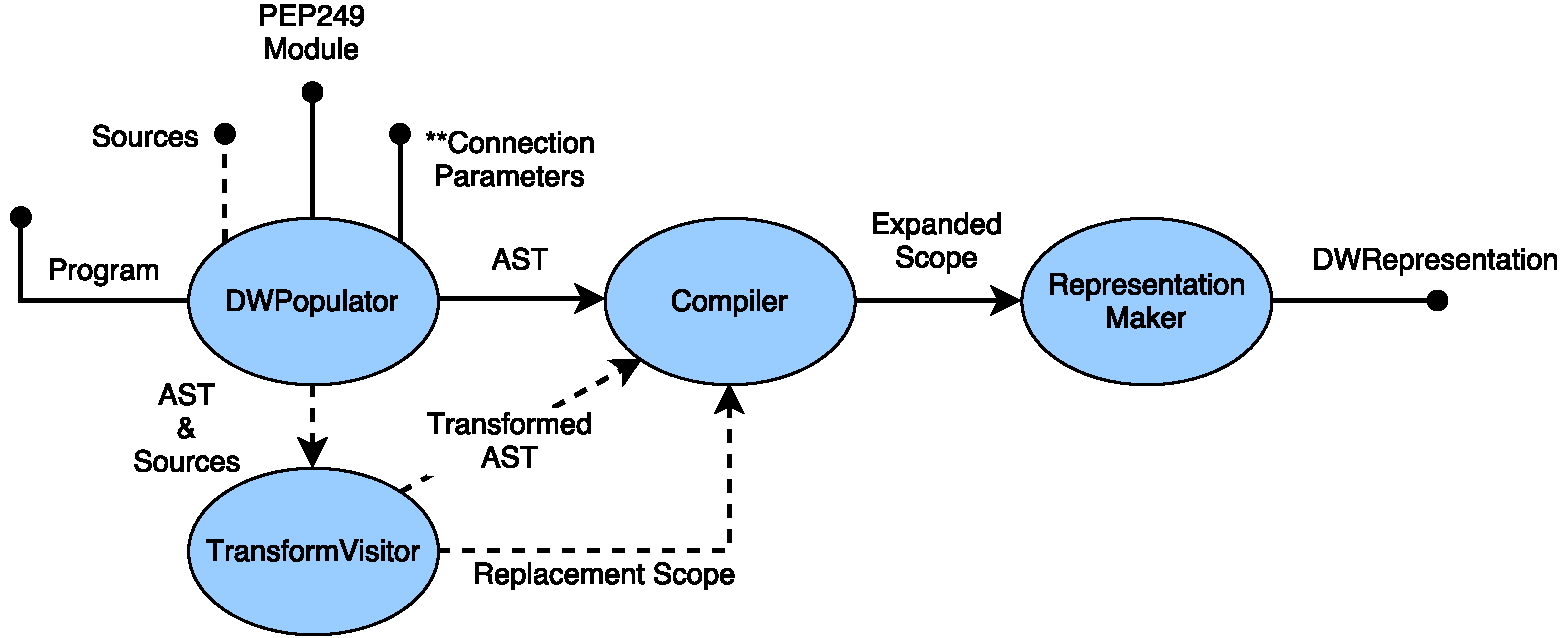
\includegraphics[width=\textwidth]{figures/reinterpreter.pdf}
\caption{Data flow diagram of the DWPopulator. The dotted lines are an alternative path, used of we decide to replace sources and DW in the program.}
\label{fig:reinterpreter}
\end{figure*}
\section{DWPopulator}\label{sec:dwpopulator}

In this section we describe the implementation of the DWPopulator component. Its is used to populate a DW using a pygrametl test program. After program execution it creates and returns a DWRepresentation object. This object is used by the predicates to gain access to DW tables and metadata. On \cref{fig:reinterpreter} is a dataflow diagram, which illustrates the flow of data through the DWPopulator. Please note that this depiction is somewhat abstracted from the actual implementation to ease explanation. In the following subsections, we describe each of the four sub-components shown on the figure. Following this, we describe what restrictions the component operates according to.

\subsection{TransformVisitor}
Before execution of the pygrametl test program, testers may choose to dynamically replace the program's hardcoded sources and DW. If they opt to do this, the TransformVisitor class is used. Otherwise the component is skipped.
The TransformVisitor takes as input the abstract syntax tree (AST) of the pygrametl program being tested, along with the test sources and DW, which we wish to use as replacements. The component walks over the AST of the pygrametl program, replacing the program's connections with those given by the tester. It inherits from ast.NodeVisitor and overwrites the visit\_Call method. This method is called, when a call node implementing a call to a method or function is encountered. The overwritten method is shown below:

\insertcodefile{CallNode.py}{The visit\_Call method of TransformVisitor}

The method only reacts to certain pygrametl method calls. After extracting the name of the method being called, we react if the name is contained in either \texttt{ATOMIC\_SOURCES} or \texttt{WRAPPERS}.

\texttt{ATOMIC\_SOURCES} is a list of the non-aggregate sources SQLSource, CSVSource and TypedCVSSource. All other sources from pygrametl.sources are aggregates of these three. Thus there is no reason to react to these. If the method name is contained within \texttt{ATOMIC\_SOURCES}, it means that a non-aggregate source is being instantiated. One of the parameters used for such an instantiation is a connection object. By replacing this with the connection object of a test source, we force the non-aggregated source to point at the test data. This means that the object can now be used to access test data, rather than the data it was hardcoded to do. The replacement process itself consists of replacing the hardcoded connection parameter with a dummy key from the replacement scope. For the first source encountered the key will be \texttt{\_\_1\_\_}, the second \texttt{\_\_2\_\_} and so on. These will later be used as identifiers, when executing the AST.

WRAPPERS contains only ConnectionWrapper from pygrametl.init. This is the class used to access DWs with pygrametl. Once the instantiation of a ConnectionWrapper is encountered, we simply replace its connection parameter with the key \texttt{\_\_0\_\_}. We also set a flag that makes sure that we raise an exception if another ConnectionWrapper is encountered. We do this to restrict \FW{} to only work with pygrametl programs that function on a single DW.

Once the entire tree has been walked, a transformed AST has been produced. We then create a replacement scope, \texttt{\_\_0\_\_} points to the DW connection and \texttt{\_\_1\_\_}, \texttt{\_\_2\_\_}, etc, points to their corresponding source connections. The transformed AST and the replacement scope is then sent to compilation.

\subsection{Compiler}
In this component we compile and execute the pygrametl program. If we used the TransformVisitor, we compile the transformed AST and execute it using the replacement scope as local scope. Otherwise, we simply compile the regular AST, and execute it with an empty local scope. In both cases, this is done with calls to the built-in python functions; compile and exec. In python, a scope is given by a dictionary, where keys are variable names paired with object references. In the case that we used TransformVisitor, we replaced the connecting objects in the transformed AST with keys from our own scope. By executing using the replacement scope, we force the program to use the test objects found in that scope. Thus we overwrite the hardcoded sources and DW from the program. Once the AST has been executed in either case, the test DW will be populated, and whatever local scope we used will have been expanded with the variables found in the executed pygrametl program. The expanded scope is sent to the RepresentationMaker. After execution we also make sure to reestablish connection to the test DW, in case it was closed during execution.

\subsection{RepresentationMaker}\label{ssec:Representation}
Using the expanded scope, the RepresentationMaker accesses all Dimension and FactTable objects instantiated through the execution of the pygrametl program. From this, it creates a DWRepresentation object that allows for easy access to all the tables of the DW along with their metadata. It begins by instantiating the RepresentationMaker, then calling its run method to create the DWRepresentation object. This method can be seen below:

\insertcodefile{representation_maker.py}{The run method of the representation\_maker class}

In this method we access the \texttt{\_alltables} list from our scope. Every pygrametl Dimension and FactTable object instantiated during execution of the pygrametl program is logged in this list. Once acquired we iterate over the list and create a representation object for each table. \texttt{check\_table\_type} is a method that returns true, if the table in question has a type contained in a given list. \texttt{DIM\_CLASSES} contains the class names of all non-aggregate Dimension classes from \texttt{pygrametl.tables}. Similarly \texttt{FT\_CLASSES} contains all non-aggregate fact table classes with the exception of SubprocessFactTable. Once the type of a table has been identified relevant metadata such as table name and keys are extracted from the object and used to instantiate a DimensionRepresentation or FactTableRepresentation respectively and stored in a list. After iteration we identify all SnowflakedDimension objects in our scope and store them in a list. These provide some assistance in discovering the structure of the DW. Afterwards the DWRepresentation object is instantiated with the two lists of tables, the list of SnowflakedDimensions and the PEP249 connection object connecting to the DW.

Once instantiated, the DWRepresentation is returned to be used by the predicates and the reinterpretation process is completed.

\subsection{Restrictions}
In this section we describe the restrictions of the DWPopulator. 

The dynamic alteration of code can become rather complex, if each edge case is considered. Thus, we decide to restrict the format of pygrametl programs that can be run through TransformVisitor. As mentioned previously, the program may only function on a single DW. We make this restriction as it makes implementation easier, while the use of more than one DW is uncommon. As we replace connections by walking over the AST, pygrametl programs may not instantiate several source or table objects through iteration. This is because, an AST walker only moves over the code within a loop a single time. Finally, the instantiation of pygrametl sources and tables may only occur in the script from which the AST is created. Imports are still usable, but because the AST walker only traverses the given script, replacements will not be performed inside imported modules.

In the RepresentationMaker we restrict ourselves from extracting metadata from instantiations of the SubprocessFactTable class. This class is used to write data to some sub processes such as a bulkloader. We ignore it, as it does not contain the needed metadata such as a table name

 All of these restrictions can be circumvented by not performing replacements of sources and DW. 

